% Experiment 02: the DIT mode-placement crossover, on both instruments.
%
% Preamble needs:  \usepackage{graphicx}  \usepackage{subcaption}
%
% The two panels are 3.35in wide each, so the pair wants a FULL-WIDTH float. On
% a USENIX-style 7in textwidth 0.49\textwidth is 3.43in and they fit side by
% side with room for \hfill. In a single 3.33in column, stack them instead --
% see the note at the bottom of this file.
%
% \includegraphics carries NO width= on purpose. The panels are drawn at their
% final size with 9pt type, and scaling them to fit a box would scale the type
% with them: at 0.49\textwidth the boxes are already within 3% of the natural
% width, so leaving them unscaled keeps 9pt at 9pt.
%
% Both panels are generated by
%   utils/dit_host_screening/signed_lookup/fig_exp02_silicon.py
% from the committed CSVs and nothing else. Do not edit the PDFs.
\begin{figure*}[t]
  \centering
  
\includegraphics{figures/crossover-panel-legend}\\[-2pt]
  \begin{subfigure}[t]{0.49\textwidth}
    \centering
    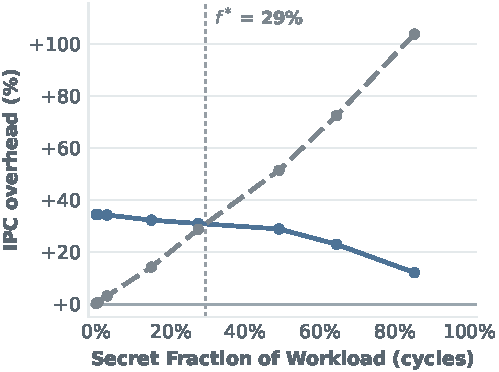
\includegraphics{figures/crossover-panel-a-m4}
    \caption{Apple M4, shipping silicon. $f^* = 29.3\%$.}
    \label{fig:xover-m4}
  \end{subfigure}\hfill
  \begin{subfigure}[t]{0.49\textwidth}
    \centering
    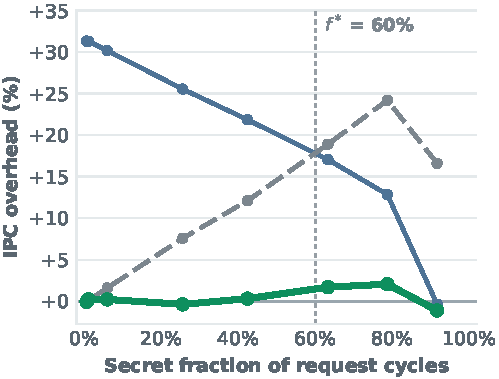
\includegraphics{figures/crossover-panel-b-gem5}
    \caption{gem5 Neoverse-V2 FDP. $f^* = 60.0\%$.}
    \label{fig:xover-gem5}
  \end{subfigure}
  \caption{%
    \textbf{Where hand placement stops paying, on one microbenchmark and two
    machines.} A request is a public lookup lane of $L$ dependent loads and one
    AES-256-GCM call over 64 secret bytes; sweeping $L$ sweeps the secret
    fraction $f$ on the $x$ axis. Blanket \texttt{PSTATE.DIT} costs the public
    lane its load-value predictions, so it gets dearer as $f$ falls; Apple's
    bracket at the crypto call pays a fixed bill per call, so it gets cheaper.
    $f^*$ is where they cross, and it is the deployment decision. $y$ is IPC
    overhead against an unhardened build, each bracket arm measured against an
    instruction-matched NOP twin.
    %
    \emph{The two $y$ ranges differ, $+105\%$ against $+35\%$, and that is a
    result rather than a plotting choice}: the same bracket costs
    333--710\,cycles per request on the M4 against 206--351 in the model, over a
    request 3.6$\times$ shorter, so it is 106\% of a secret-heavy request on
    hardware and 18\% of one in simulation. The simulator is optimistic about
    hand placement by roughly a factor of two in secret fraction. The dashed
    curve is the simulator's own renamed switch design, which never crosses.%
  }
  \label{fig:xover}
\end{figure*}

% ---------------------------------------------------------------------------
% SINGLE-COLUMN variant: same three files, stacked, in a \columnwidth float.
% Replace figure* above with this if the pair has to live in one column.
%
% \begin{figure}[t]
%   \centering
%   
\includegraphics[width=\columnwidth]{figures/crossover-panel-legend}
%   \begin{subfigure}{\columnwidth}
%     \centering
%     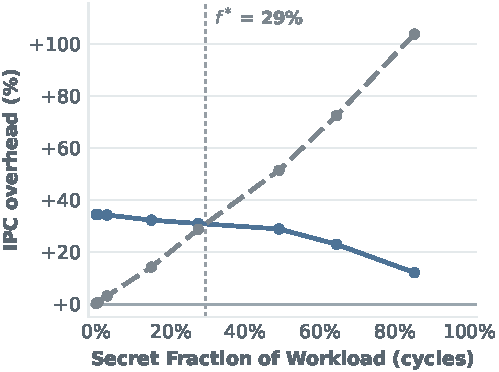
\includegraphics[width=\columnwidth]{figures/crossover-panel-a-m4}
%     \caption{Apple M4, shipping silicon.}
%   \end{subfigure}
%   \begin{subfigure}{\columnwidth}
%     \centering
%     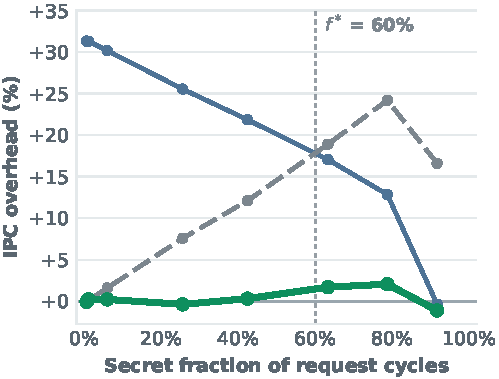
\includegraphics[width=\columnwidth]{figures/crossover-panel-b-gem5}
%     \caption{gem5 Neoverse-V2 FDP.}
%   \end{subfigure}
%   \caption{...}
% \end{figure}
